\documentclass[11pt,a4paper,twoside,pdf]{article}

% Paquetes (añade otros si los necesitas):
\usepackage{latexsym}
\usepackage[utf8x]{inputenc}
\usepackage{soul}
\usepackage{array}
\usepackage{amsmath}
\usepackage{amssymb}
\usepackage{marvosym}
\usepackage{epsfig}
\usepackage{graphics}
\usepackage{amsfonts}
\usepackage{xspace}
\usepackage{color}
\usepackage{booktabs}
\usepackage{xtab}
\usepackage[colorlinks=true,urlcolor=blue,linkcolor=blue,citecolor=blue]{hyperref}
\numberwithin{equation}{section}

% Fuente: palatino
\usepackage[sc]{mathpazo}
\linespread{1.05}

% TFG en inglés:
%\usepackage[english]{babel} 
%\addto\captionsenglish{\renewcommand{\chaptername}{}}

% TFG en español:
\usepackage[spanish,es-nodecimaldot,es-tabla,es-lcroman,es-nosectiondot,
            es-noindentfirst]{babel}
\renewcommand\spanishchaptername{}

% Formato de la página:
\usepackage{fancyhdr}
\usepackage[top=2.88cm,bottom=2.97cm,left=2.95cm,right=2.95cm]{geometry}
\setlength{\parskip}{0.1cm}

% Pon aquí tus definiciones:

\newcommand{\dis}{\displaystyle}
\sodef\an{}{.2em}{1em plus1em}{2em plus.1em minus.1em}

\begin{document}

% Portada %%%%%%%%%%%%%%%%%%%%%%%%%%%%%%%%%%%%%%%%%%%%%%%%%%%%%%%%%%%%%%%%%%%%%%

\pagestyle{empty}


\noindent
\begin{tabular}{r}

\includegraphics[width=8.8cm]{escudoUGRmonocromo.png} \\[-1.8ex]
\hspace{31mm}\vspace{-8mm}
\begin{tabular}{c}
\hline\\[-1ex]\hskip-2mm
{\bf Facultad de Ciencias}\hspace{18mm}
\end{tabular}
\end{tabular}

{\large
\vspace{30mm}
\hspace{25mm}
\begin{tabular}{l}
\an{GRADO EN FISICA}
\end{tabular}

\vspace{45mm}
\hspace{25mm}
\begin{tabular}{l}
\an{TRABAJO FIN DE GRADO}
\\[1.5ex]
\an{\LARGE\bf IMPLEMENTACI\'ON DE }
\\
\an{\LARGE\bf M\'ETODOS}
\\
\an{\LARGE\bf EN DIFERENCIAS FINITAS }
\\
\an{\LARGE\bf EN GPUs}
\end{tabular}

\vfill
\hspace{25mm}
\begin{tabular}{l}
Presentado por:
\\
{\bf D. JUAN JOS\'E SALAZAR L\'OPEZ}
\\[3ex]
Curso Académico 2021/2022
\end{tabular}
}


\newpage

\begin{center}

{\bf Resumen}
\bigskip

\begin{minipage}{0.8\linewidth}
El método numérico de las diferencias finitas dependientes del tiempo (FDTD) se usa como herramienta para la resolución de ecuaciones diferenciales de primer orden.  Este cobra especial importancia en la electrodinámica computacional dado que nos permite resolver las ecuaciones de Maxwell realizando algoritmos con los que calcular punto a punto los valores del campo electromagnético. Generalmente se implementan estos algoritmos usando la potencia de cálculo que nos proporcionan las CPUs, en este TFG se ha generado un algoritmo 'open source' en cuda para exponer las ventajas que se obtienen al implementar este método usando el poder de paralelización que nos proporcionan las GPUs. 
\end{minipage}

\vfill

{\bf Abstract} 
\bigskip

\begin{minipage}{0.8\linewidth}
FDTD method implementation for the resolution of one order diferential equation in GPUs to achieve an improvement in the calculus time.
\end{minipage}

\vfill

\end{center}

% Indice %%%%%%%%%%%%%%%%%%%%%%%%%%%%%%%%%%%%%%%%%%%%%%%%%%%%%%%%%%%%%%%%%%%%%%%
\newpage

\tableofcontents

% Texto %%%%%%%%%%%%%%%%%%%%%%%%%%%%%%%%%%%%%%%%%%%%%%%%%%%%%%%%%%%%%%%%%%%%%%%%
\newpage

\pagestyle{fancy}
\fancyhead[RO,LE]{\leftmark}
\fancyhead[LO,RE]{\thepage}
\fancyfoot{}

\section{Introducción}
El método numérico de las diferencias finitas es usado en muchos campos para la resolución de ecuaciones diferenciales de primer orden. En particular, el método de la diferencia central finita cobra especial importancia en la electrodinámica computacional donde se emplea para resolver las ecuaciones de Maxwell en el dominio del tiempo, discretizando tiempo y el espacio para poder implementar la solución en un algoritmo.
Actualmente su uso está muy extendido ya que posibilita el estudio de la propagación de señales electromagnéticas por diversos medios. En particular puede usarse para determinar la radiación que actúa sobre una cabeza humana producida por un teléfono móvil o la propagación de una señal en el uso de radares marítimos entre otras aplicaciones.

Desde que se desarrolló el método y se generaron los primero algoritmos se ha hecho uso del poder de cómputo que nos proporcionan las CPUs, el cual ha ido creciendo con el paso de los años. No obstante, al aumentar la dimensión espacial en el modelo también aumenta el tiempo necesario para obtener la solución dado que se debe calcular punto a punto los valores de los campos al aplicar el método. Este problema puede solventarse haciendo uso del poder de paralelización que nos ofrecen las tarjetas gráficas (GPUs), pudiendo hacer simultaneamente, hasta cierto límite, todas las operaciones que se realizan punto a punto en la dimensión espacial. Proceso que se consigue implementando los algoritmos FDTD en el lenguaje CUDA, con el cual podemos especificar punto a punto el cálculo a realizar por cada hilo dentro de la GPU.

En este TFG el autor ha desarrollado varios códigos en CUDA de libre uso para la resolución de las ecuaciones de Maxwell aplicando el método FDTD en dos dimensiones. Los códigos generados pueden encontrarse en el siguiente repositorio de github:

https://github.com/juanjo1213/TFG-FDTD

En el mismo pueden encontrarse los códigos para la solución en 2D implementada en la cpu y en la gpu, siendo todos los algoritmos del repositorio de libre uso.

\newpage




\section{Metodología}
El método numé rico de las diferencias finitas se emplea en la resolución de ecuaciones diferenciales de primer orden, en particular, el método de la diferencia central finita se basa en aproximar de forma sencilla la derivada de una función en un punto como la diferencia de dicha función evaluada en dos puntos equidistantes al mismo. Haciendo uso del desarrollo en serie de Taylor y aproximando a segundo orden obtenemos:

\begin{equation}
f(x+h)=y(x)+hy^\prime(x)+\frac{h^3}{2}y^{\prime\prime}(x)+\frac{h^3}{6}y^{\prime\prime\prime}(x)
\end{equation}

\begin{equation}
f(x-h)=y(x)-hy^\prime(x)+\frac{h^3}{2}y^{\prime\prime}(x)+\frac{h^3}{6}y^{\prime\prime\prime}(x)
\end{equation}

\begin{equation}
y\prime(x)=\frac{y(x+h)-y(x-h)}{2h}+O(h^2)
\end{equation}

Donde hemos despejado el valor de la derivada de la función en un punto mediante su desarrollo en serie en (x+h) y (x-h).

Recordando la expresión de las ecuaciones de Maxwell para el campo electromagnético, haciendo uso del vector campo D.

\begin{equation}
\frac{\partial D}{\partial t}=\nabla \times H
\end{equation}

\begin{equation}
D(\omega)=\varepsilon_{0}\varepsilon^*_{r}(\omega)E(\omega)
\end{equation}

\begin{equation}
\frac{\partial H}{\partial t}=-\frac{1}{\mu_{0}}\nabla \times E
\end{equation}

Podemos observar que están expresadas en el dominio de la frecuencia para poder aplicarlas a medios cuya constante dieléctrica dependa de la misma. Resaltar que $\varepsilon_{0}$ y $\varepsilon_{r}$ corresponden a las constantes dieléctricas del vacío y del medio respectivamente, y $\mu_{0}$ es la permeabilidad magnética del vacío.


Para simplificar el formalismo es conveniente normalizar las ecuaciones haciendo uso de las constantes dieléctrica y permeabilidad magnética del vacío.
\begin{equation}
\tilde{E}=\sqrt{\frac{\varepsilon_{0}}{\mu_{0}}}E
\end{equation}

\begin{equation}
\tilde{D}=\frac{1}{\sqrt{\varepsilon_{0}\mu_{0}}}D
\end{equation}

De este modo podemos expresar las ecuaciones de Maxwell para el campo electromagnético como:

\begin{equation}
\frac{\partial \tilde{D}}{\partial t}=-\frac{1}{\sqrt{\varepsilon_{0}\mu_{0}}}\nabla \times H
\end{equation}

\begin{equation}
\tilde{D}(\omega)=\varepsilon^*_{r}(\omega)\tilde{E}(\omega)
\end{equation}

\begin{equation}
\frac{\partial H}{\partial t}=-\frac{1}{\sqrt{\varepsilon_{0}\mu_{0}}}\nabla \times E
\end{equation}


En $\mathbb R^{3}$ tenemos 3 componentes para el campo eléctrico y 3 para el magnético $\tilde{E}_{x}$, $\tilde{E}_{y}$, $\tilde{E}_{z}$, $H_{x}$, $H_{y}$, $H_{z}$, por lo que, si queremos aplicar un modelo en dos dimensiones debemos elegir uno de los dos grupos de tres vectores, (i) el transversal magnético, formado por $\tilde{E}_{z}$, $H_{x}$, $H_{y}$, o (ii) el transversal eléctrico, compuesto por los vectores $\tilde{E}_{x}$, $\tilde{E}_{y}$ y $H_{z}$.

Usaremos el modo transversal magnético y utilizaremos directamente las letras E y D sin tildar para nombrar a las componentes normalizadas de los campos:

\begin{equation}
\frac{\partial D_{z}}{\partial t}=\frac{1}{\sqrt{\varepsilon_{0}\mu_{0}}}(\frac{\partial H_{y}}{\partial x}-\frac{\partial H_{x}}{\partial y})
\end{equation}

\begin{equation}
{D}(\omega)=\varepsilon^*_{r}(\omega)\tilde{E}(\omega)
\end{equation}

\begin{equation}
\frac{\partial H_{x}}{\partial t}=-\frac{1}{\sqrt{\varepsilon_{0}\mu_{0}}}\frac{\partial E_{z}}{\partial y}
\end{equation}

\begin{equation}
\frac{\partial H_{y}}{\partial t}=\frac{1}{\sqrt{\varepsilon_{0}\mu_{0}}}\frac{\partial E_{z}}{\partial x}
\end{equation}

Estas son las ecuaciones de una onda plana moviendose en la dirección x e y con el campo eléctrico orientado en la dirección z y el magnético en la dirección x e y. Las componentes a calcular son ecuaciones diferenciales de primer orden, por lo que, aplicando el método de la diferencia central término a término obtenemos.

\begin{equation}
\begin{split}
\frac{D^{n+1/2}_{z}(i,j)-D^{n-1/2}_{z}(i,j)}{\Delta t}=\frac{1}{\sqrt{\varepsilon_{0}\mu_{0}}}\left[\frac{H^{n}_{y}(i+\frac{1}{2},j)-H^{n}_{y}(i-\frac{1}{2},j)}{\Delta x}\right]  \\
-\frac{1}{\sqrt{\varepsilon_{0}\mu_{0}}}\left[\frac{H^{n}_{x}(i,j+\frac{1}{2})-H^{n}_{x}(i,j-\frac{1}{2})}{\Delta x}\right] 
\end{split}
\end{equation}

\begin{equation}
\frac{H^{n+1}_{x}(i,j+\frac{1}{2})-H^{n}_{x}(i,j+\frac{1}{2})}{\Delta t}=-\frac{1}{\sqrt{\varepsilon_{0}\mu_{0}}}\left[\frac{E^{n+1/2}_{z}(i,j+1)-E^{n+1/2}_{z}(i,j)}{\Delta x}\right] 
\end{equation}

\begin{equation} 
\frac{H^{n+1}_{y}(i+\frac{1}{2},j)-H^{n}_{y}(i+\frac{1}{2},j)}{\Delta t}=\frac{1}{\sqrt{\varepsilon_{0}\mu_{0}}}\left[\frac{E^{n+1/2}_{z}(i+1,j)-E^{n+1/2}_{z}(i,j)}{\Delta x}\right] 
\end{equation}

En estas ecuaciones el tiempo se especifica con el superíndice, donde n es el paso temporal, de modo que $t=\Delta t\cdot n$, en los paréntesis especificamos los valores de i, j para determinar la posición, sin olvidar que el campo eléctrico y el magnético están intercalados en tiempo y espacio, lo cual se especifica con la suma y resta de valores $\frac{1}{2}$ en los superíndices y paréntesis. 
Asumiremos $\Delta x = \Delta y$.

Una vez se ha elegido el tamaño de celda ($\Delta x \cdot \Delta y$) podemos calcular el salto temporal como:

\begin{equation}
\Delta t=\frac{\Delta x}{2 \cdot c_{0}}
\end{equation}

Donde $c_{0}$ es la velocidad de la luz en el vacío. Recordando que $\varepsilon_{0} \mu_{0}=1/(c_{0})^2$ y teniendo en cuenta la normalización utilazada:

\begin{equation}
    \frac{\Delta t}{\sqrt{\varepsilon_{0} \mu_{0}} \Delta x}=\frac{\Delta x}{2 \cdot c_{0}}\cdot 
     \frac{1}{\sqrt{\varepsilon_{0} \mu_{0}} \Delta x}=\frac{1}{2}
\end{equation}

Lo que nos permite, junto a las expresiones discretizadas en tiempo y espacio de las ecuaciones de Maxwell, generar un algoritmo de forma sencilla para calcular los campos:

\begin{equation}
dz[i,j]=dz[i,j] + 0.5*(hy[i,j]-hy[i-1,j]-hx[i,j]+hx[i,j-1])
\end{equation}

\begin{equation}
    ez[i,j]=gaz[i,j]*dz[i,j]
\end{equation}

\begin{equation}
    hx[i,j]=hx[i,j]+0.5*(ez[i,j]-ez[i,j+1])
\end{equation}

\begin{equation}
    hy[i,j]=hy[i,j]+0.5*(ez[i+1,j]-ez[i,j])
\end{equation}

\newpage


\section{Algoritmo}
----

\begin{figure}[h]
\centering
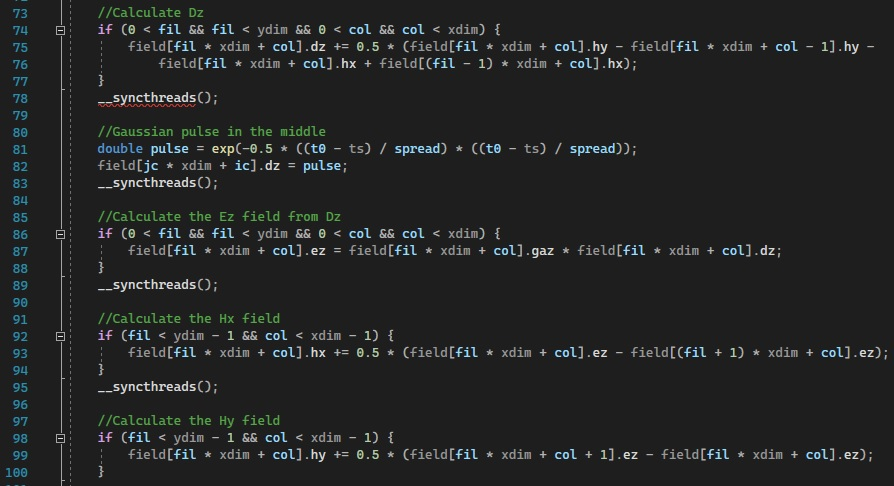
\includegraphics[width=15cm]{FD2D_Kernel_loop.jpg}				
\caption{Implementación de las ecuaciones (2.21-2.24) para el cálculo de los campos en la GPU }
\end{figure}
\noindent

\begin{figure}[h]
\centering
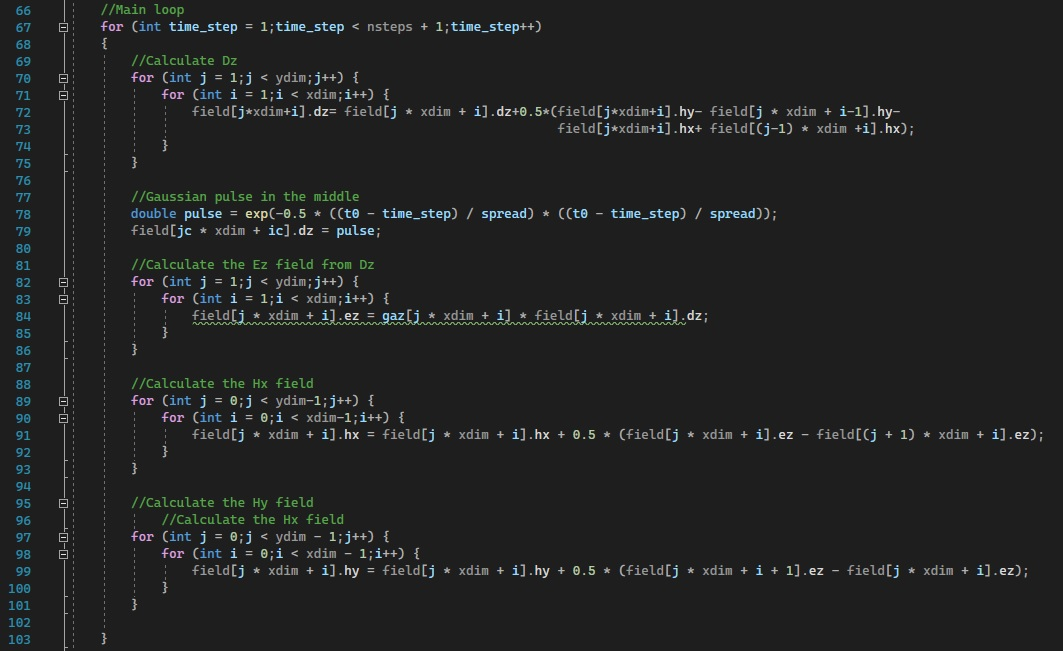
\includegraphics[width=15cm]{FD2D_Host_loop.jpg}				
\caption{Implementación de las ecuaciones (2.21-2.24) para el cálculo de los campos en la CPU }
\end{figure}
\noindent

\newpage

\section{CPU}

\newpage

\section{Resultados}

\newpage






\section{Una sección}






\section{Conclusiones}



% Referencias %%%%%%%%%%%%%%%%%%%%%%%%%%%%%%%%%%%%%%%%%%%%%%%%%%%%%%%%%%%%%%%%%
\newpage

\addcontentsline{toc}{section}{Referencias} % Elige según idioma
%\addcontentsline{toc}{section}{References} % Elige según idioma

\begin{thebibliography}{100}


 
\end{thebibliography}

\end{document}
